\documentclass{beamer}

% images
\usepackage{graphicx}
\graphicspath{ {./images/} }

\title{QR-Mixed-Reality-Framework}
\subtitle{github.com/QR-AR-Group/QR-Mixed-Reality-Framework}
\author{
  Adrian Ruppert \
  Jonathan Neidel \
  Leon Enzenberger
}
\date{July 2022}
\institute{HTW Berlin, Angewandte Informatik, AR Applications and Theoretical Foundations}
\logo{
\includegraphics[width=1cm]{htw-logo}}

% theme + color theme
\usetheme{Szeged}
\usecolortheme{whale}
% see: https://deic-web.uab.cat/~iblanes/beamer_gallery/index.html
\setbeamerfont{caption}{size=\Tiny}

\begin{document}
\frame{\titlepage}

% What will your application be about?
% Why did you decide on this specific topic?
% What will it look like? (Mockups/paper prototypes would be ideal)
% Which features will it have?
% Who will take over which parts of the development?

\section{Purpose}
\begin{frame}
	\begin{center}
		{\Huge What will your application be about?}
	\end{center}
\end{frame}
\begin{frame}
  \frametitle{Example}
  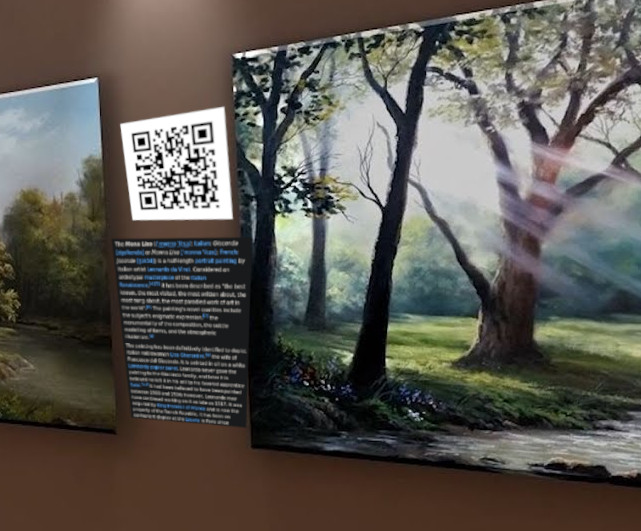
\includegraphics[width=11cm]{gallery_example}
\end{frame}

\begin{frame}
  \frametitle{QR Codes}
  QR codes with content encoded in it:
  \begin{itemize}
    \item Url
    \item Scale and relative position (to QR code)
  \end{itemize}
\end{frame}

\begin{frame}
  \frametitle{Basic functionality}

  The app will:
  \begin{itemize}
    \item Create QR codes with encoded content
    \item Read QR codes and display content
  \end{itemize}
\end{frame}

\section{Background}
\begin{frame}
	\begin{center}
		{\Huge Why did you decide on this specific topic?}
	\end{center}
\end{frame}

\begin{frame}
  \frametitle{Original Idea}

  Browse a QR codes webpage by overlaying it in AR.
\end{frame}

\begin{frame}
  \frametitle{Pivot}

  Non-interactive webpages.

  \medskip

  Fine grained control over positioning the content.
\end{frame}

\begin{frame}
  \frametitle{An Adhoc System}

  \begin{itemize}
    \item Anybody can create QR codes
    \item Anybody can read out QR codes
    \item No central server
  \end{itemize}
\end{frame}

\begin{frame}
  \frametitle{Web Content}

  Content:
  \begin{itemize}
    \item Any webpage
    \item Allows for animation, sound and video
  \end{itemize}
\end{frame}

\begin{frame}
  \frametitle{Another example}

  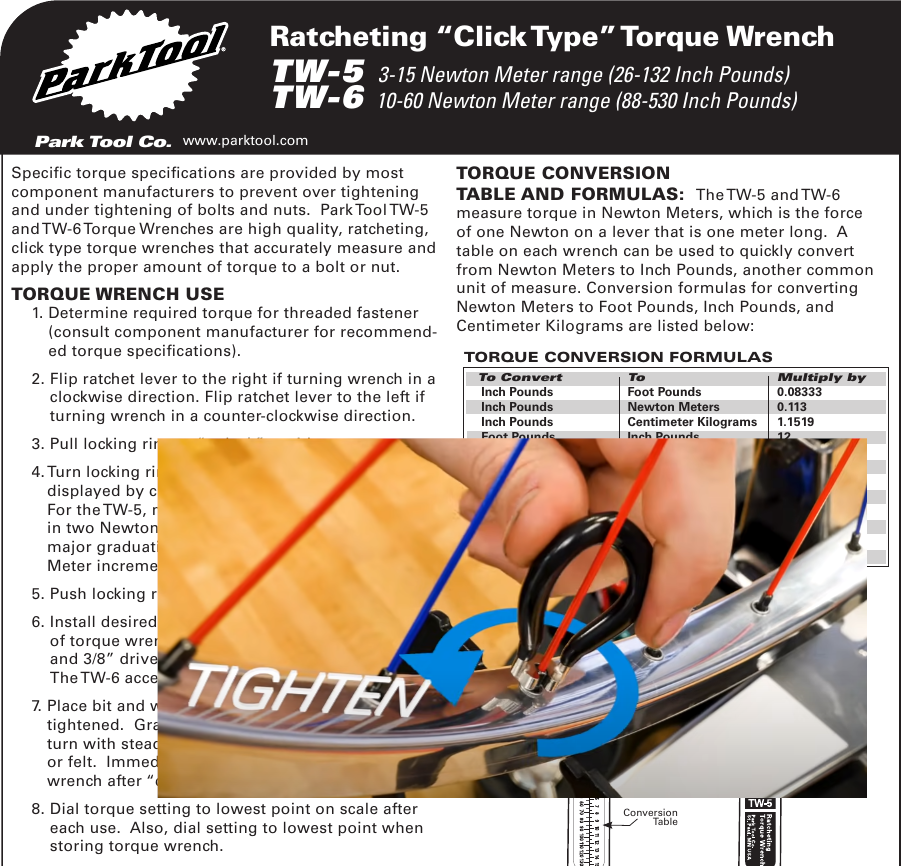
\includegraphics[height=8cm]{manual_example}
\end{frame}

\section{UI}
\begin{frame}
	\begin{center}
		{\Huge What will it look like?}
	\end{center}
\end{frame}
\begin{frame}
  \frametitle{Reading QR Code}

  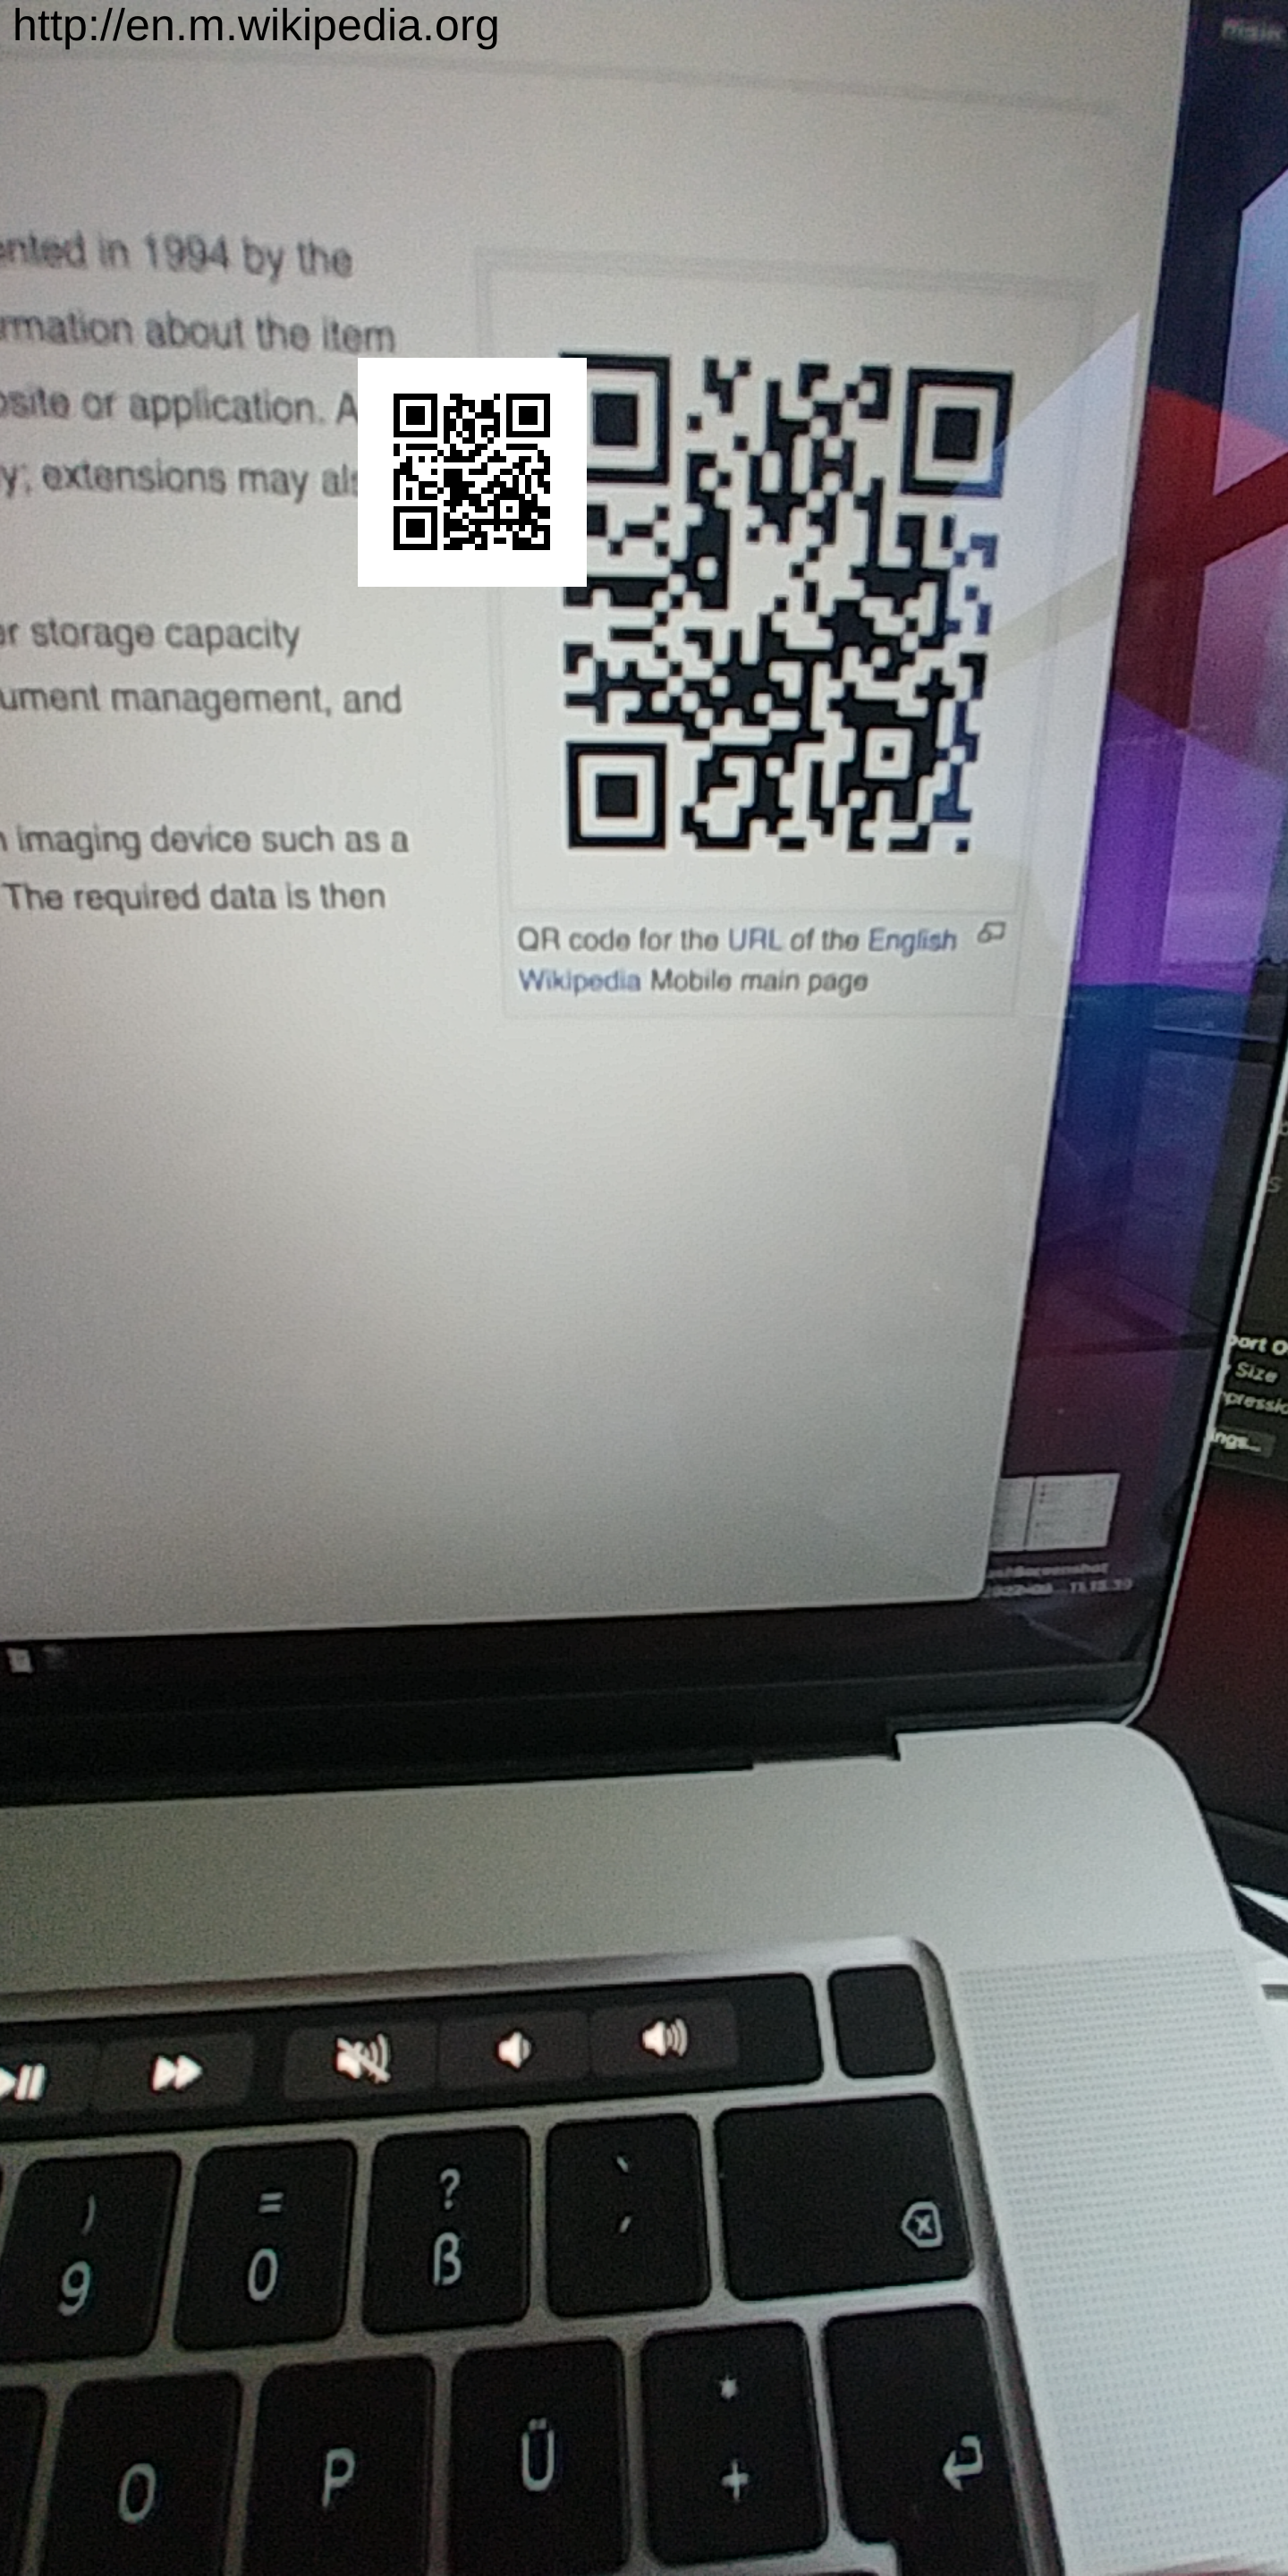
\includegraphics[height=8cm]{detect}
\end{frame}

\begin{frame}
  \frametitle{Creating QR Code Flow}

  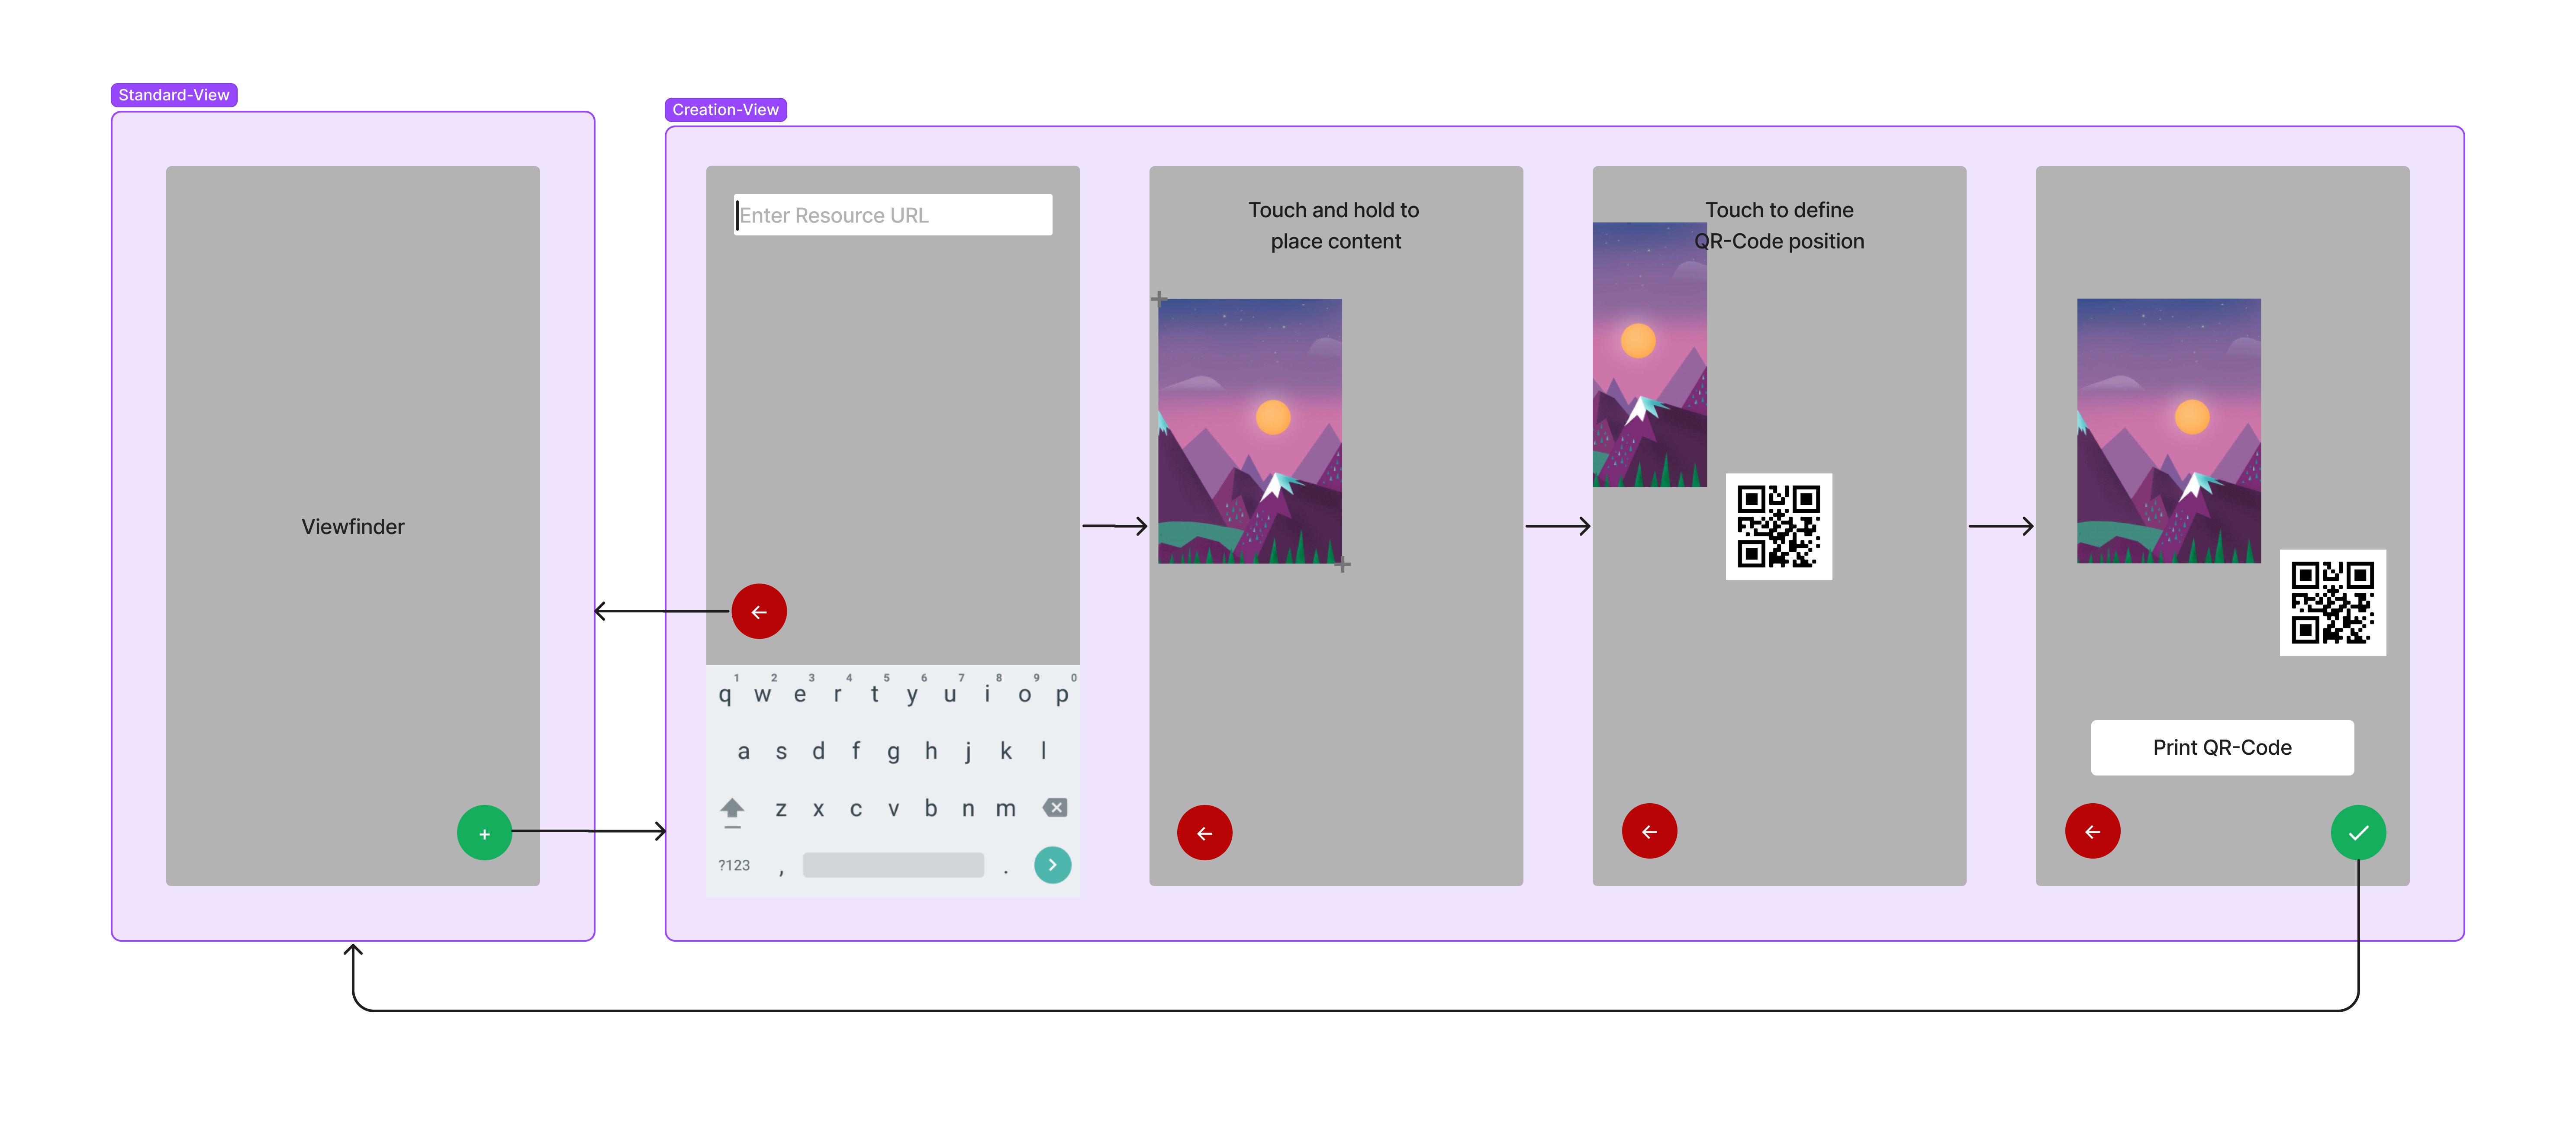
\includegraphics[width=12cm]{UI-Mockup}
\end{frame}

\begin{frame}
  \frametitle{Creating QR Code I}
  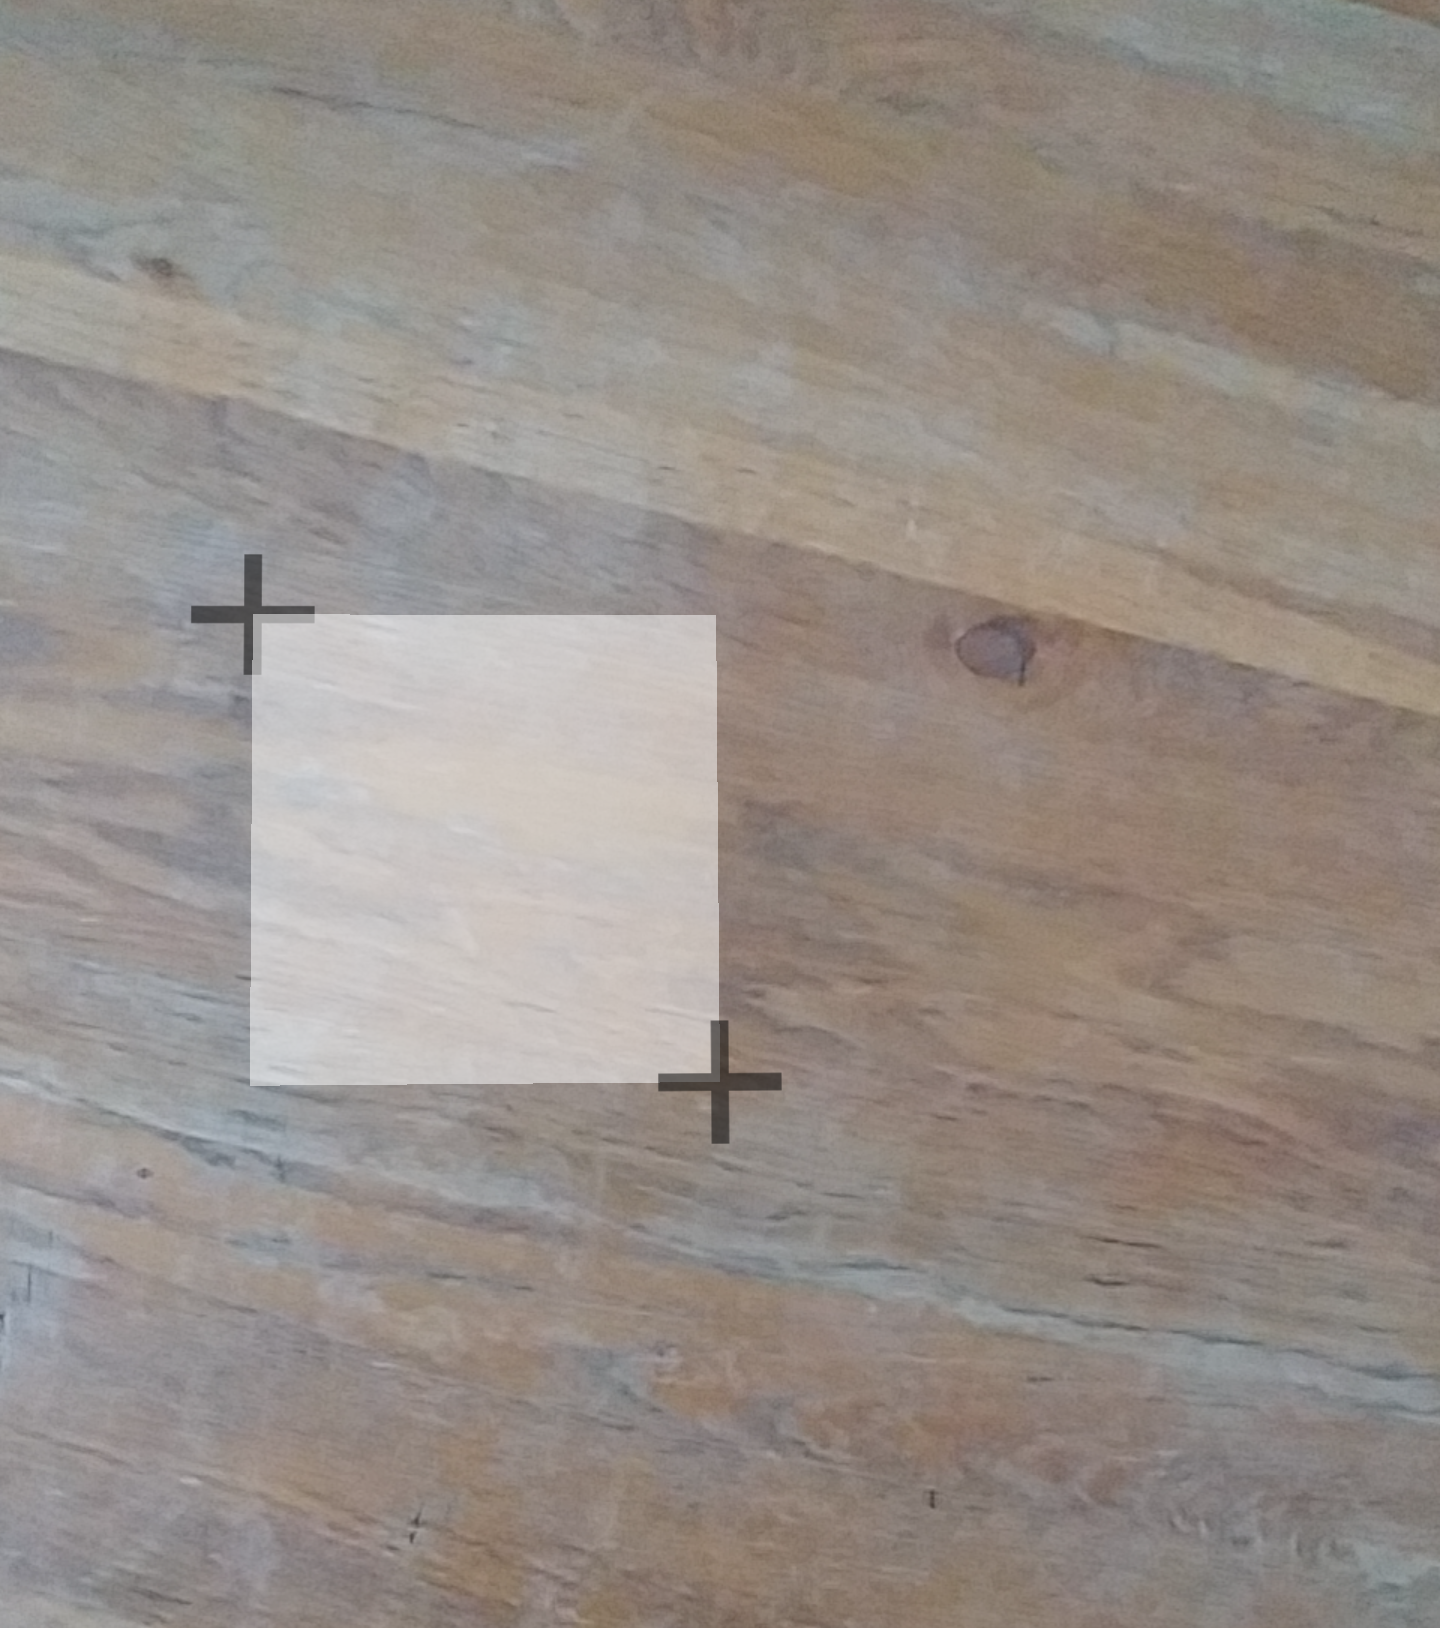
\includegraphics[height=8cm]{span}
\end{frame}

\begin{frame}
  \frametitle{Creating QR Code II}
  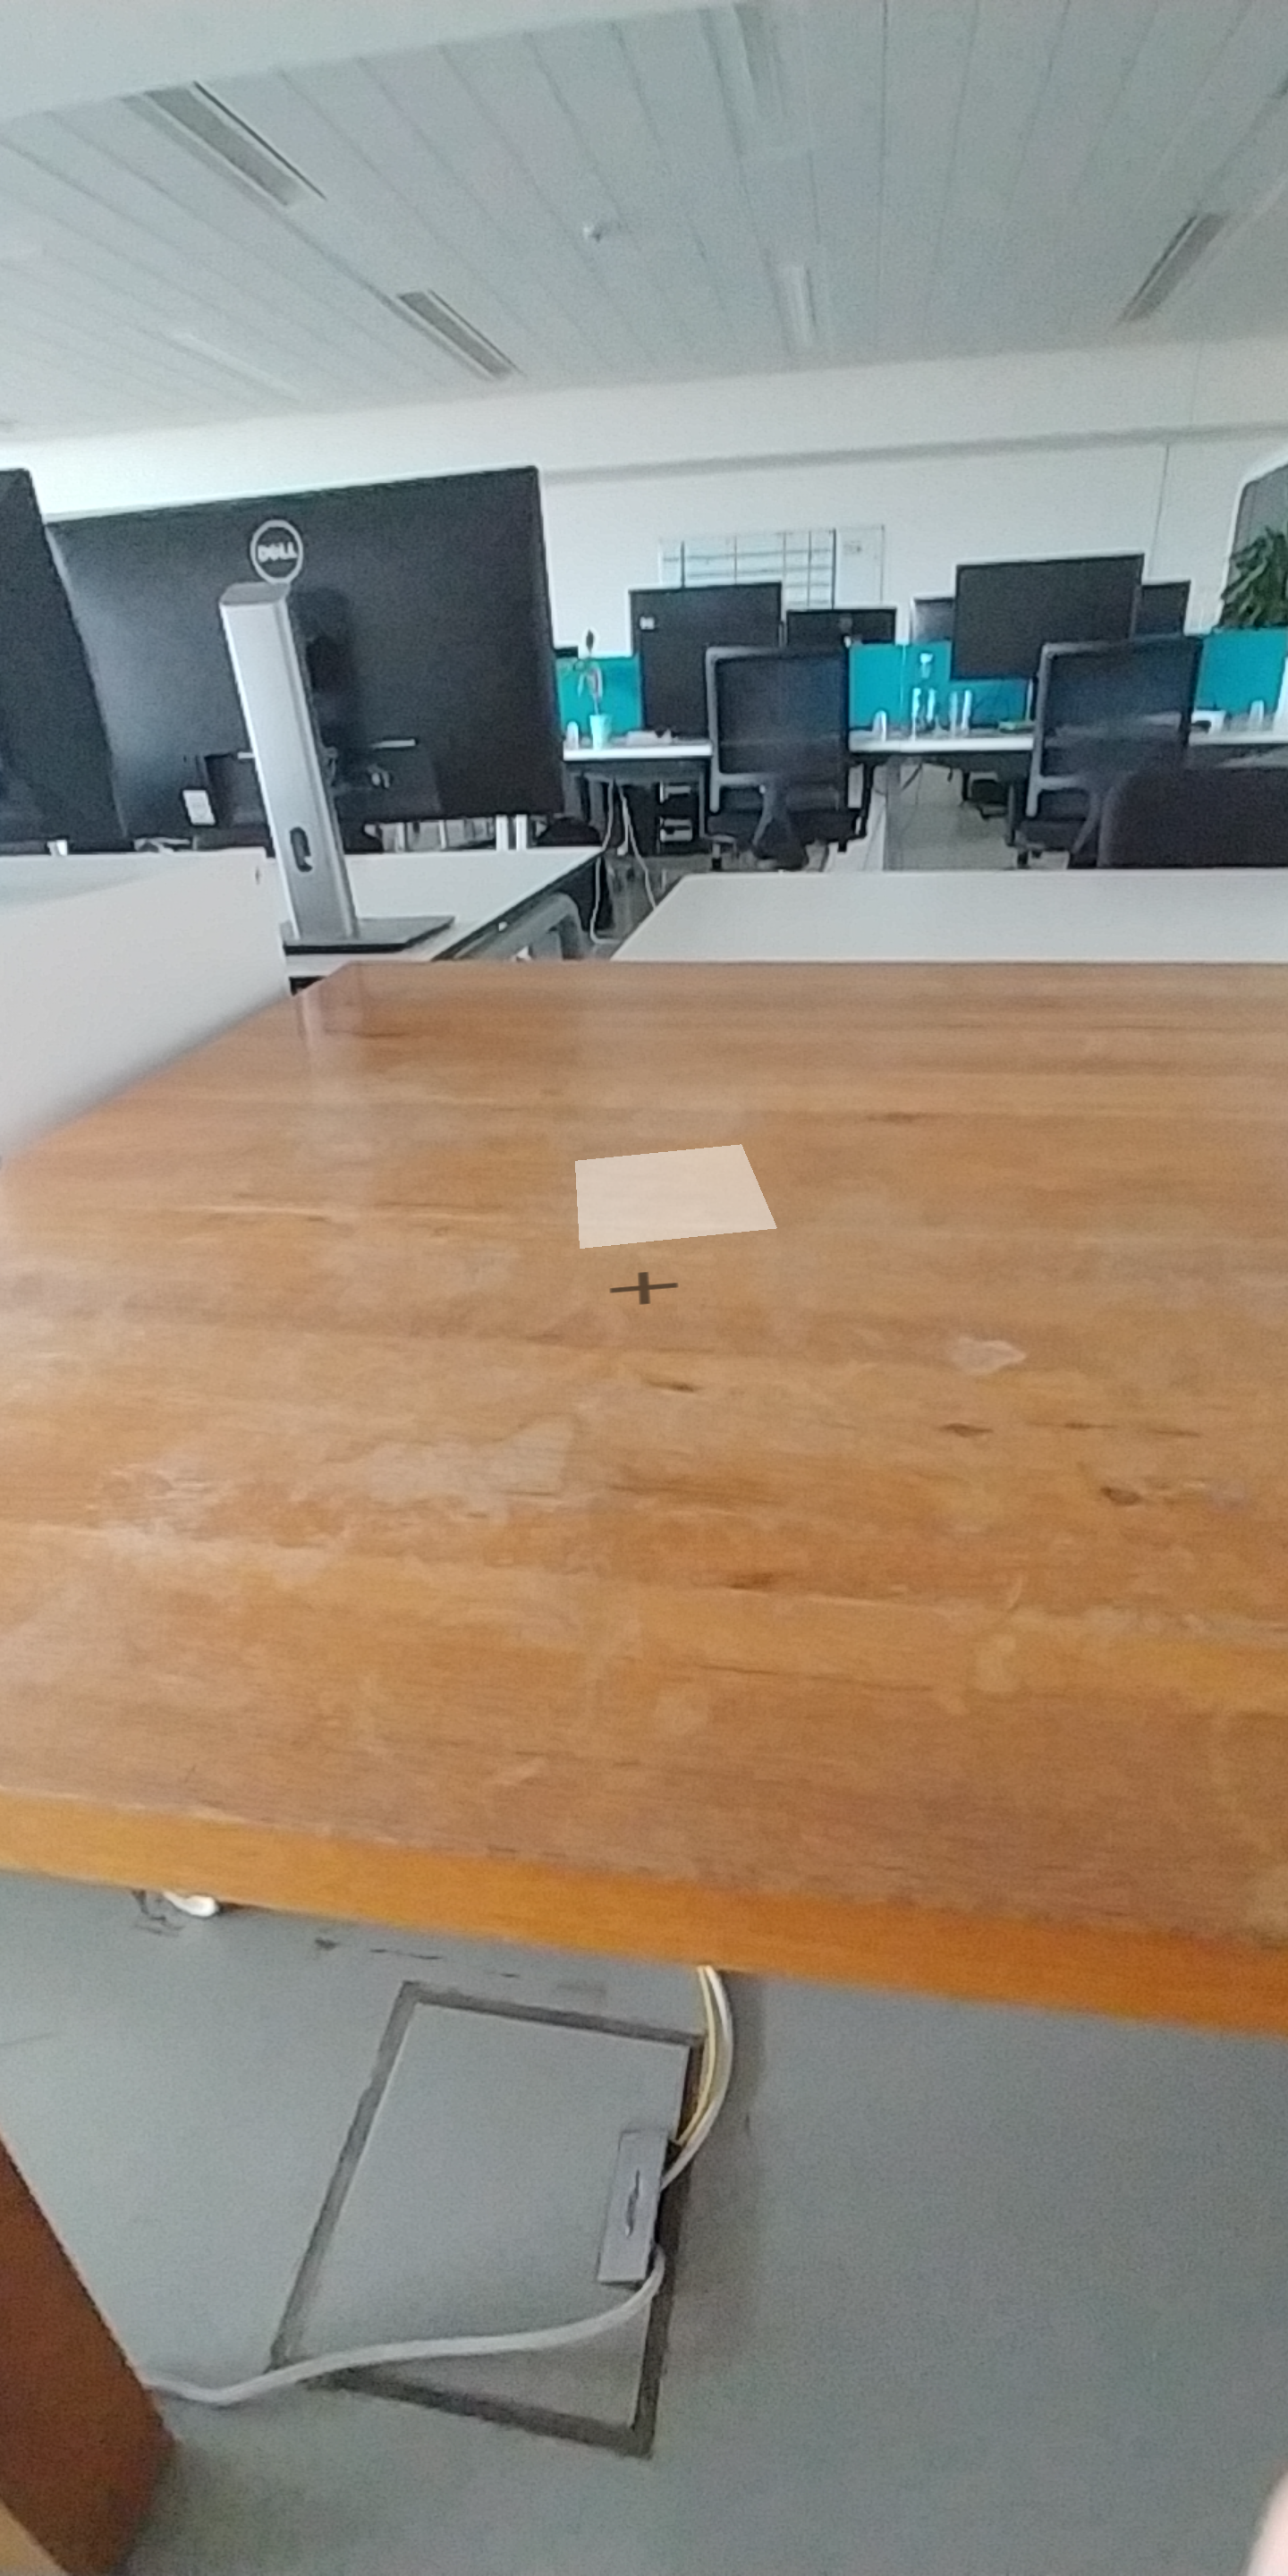
\includegraphics[height=8cm]{spanned}
\end{frame}

\begin{frame}
  \frametitle{Creating QR Code III}
  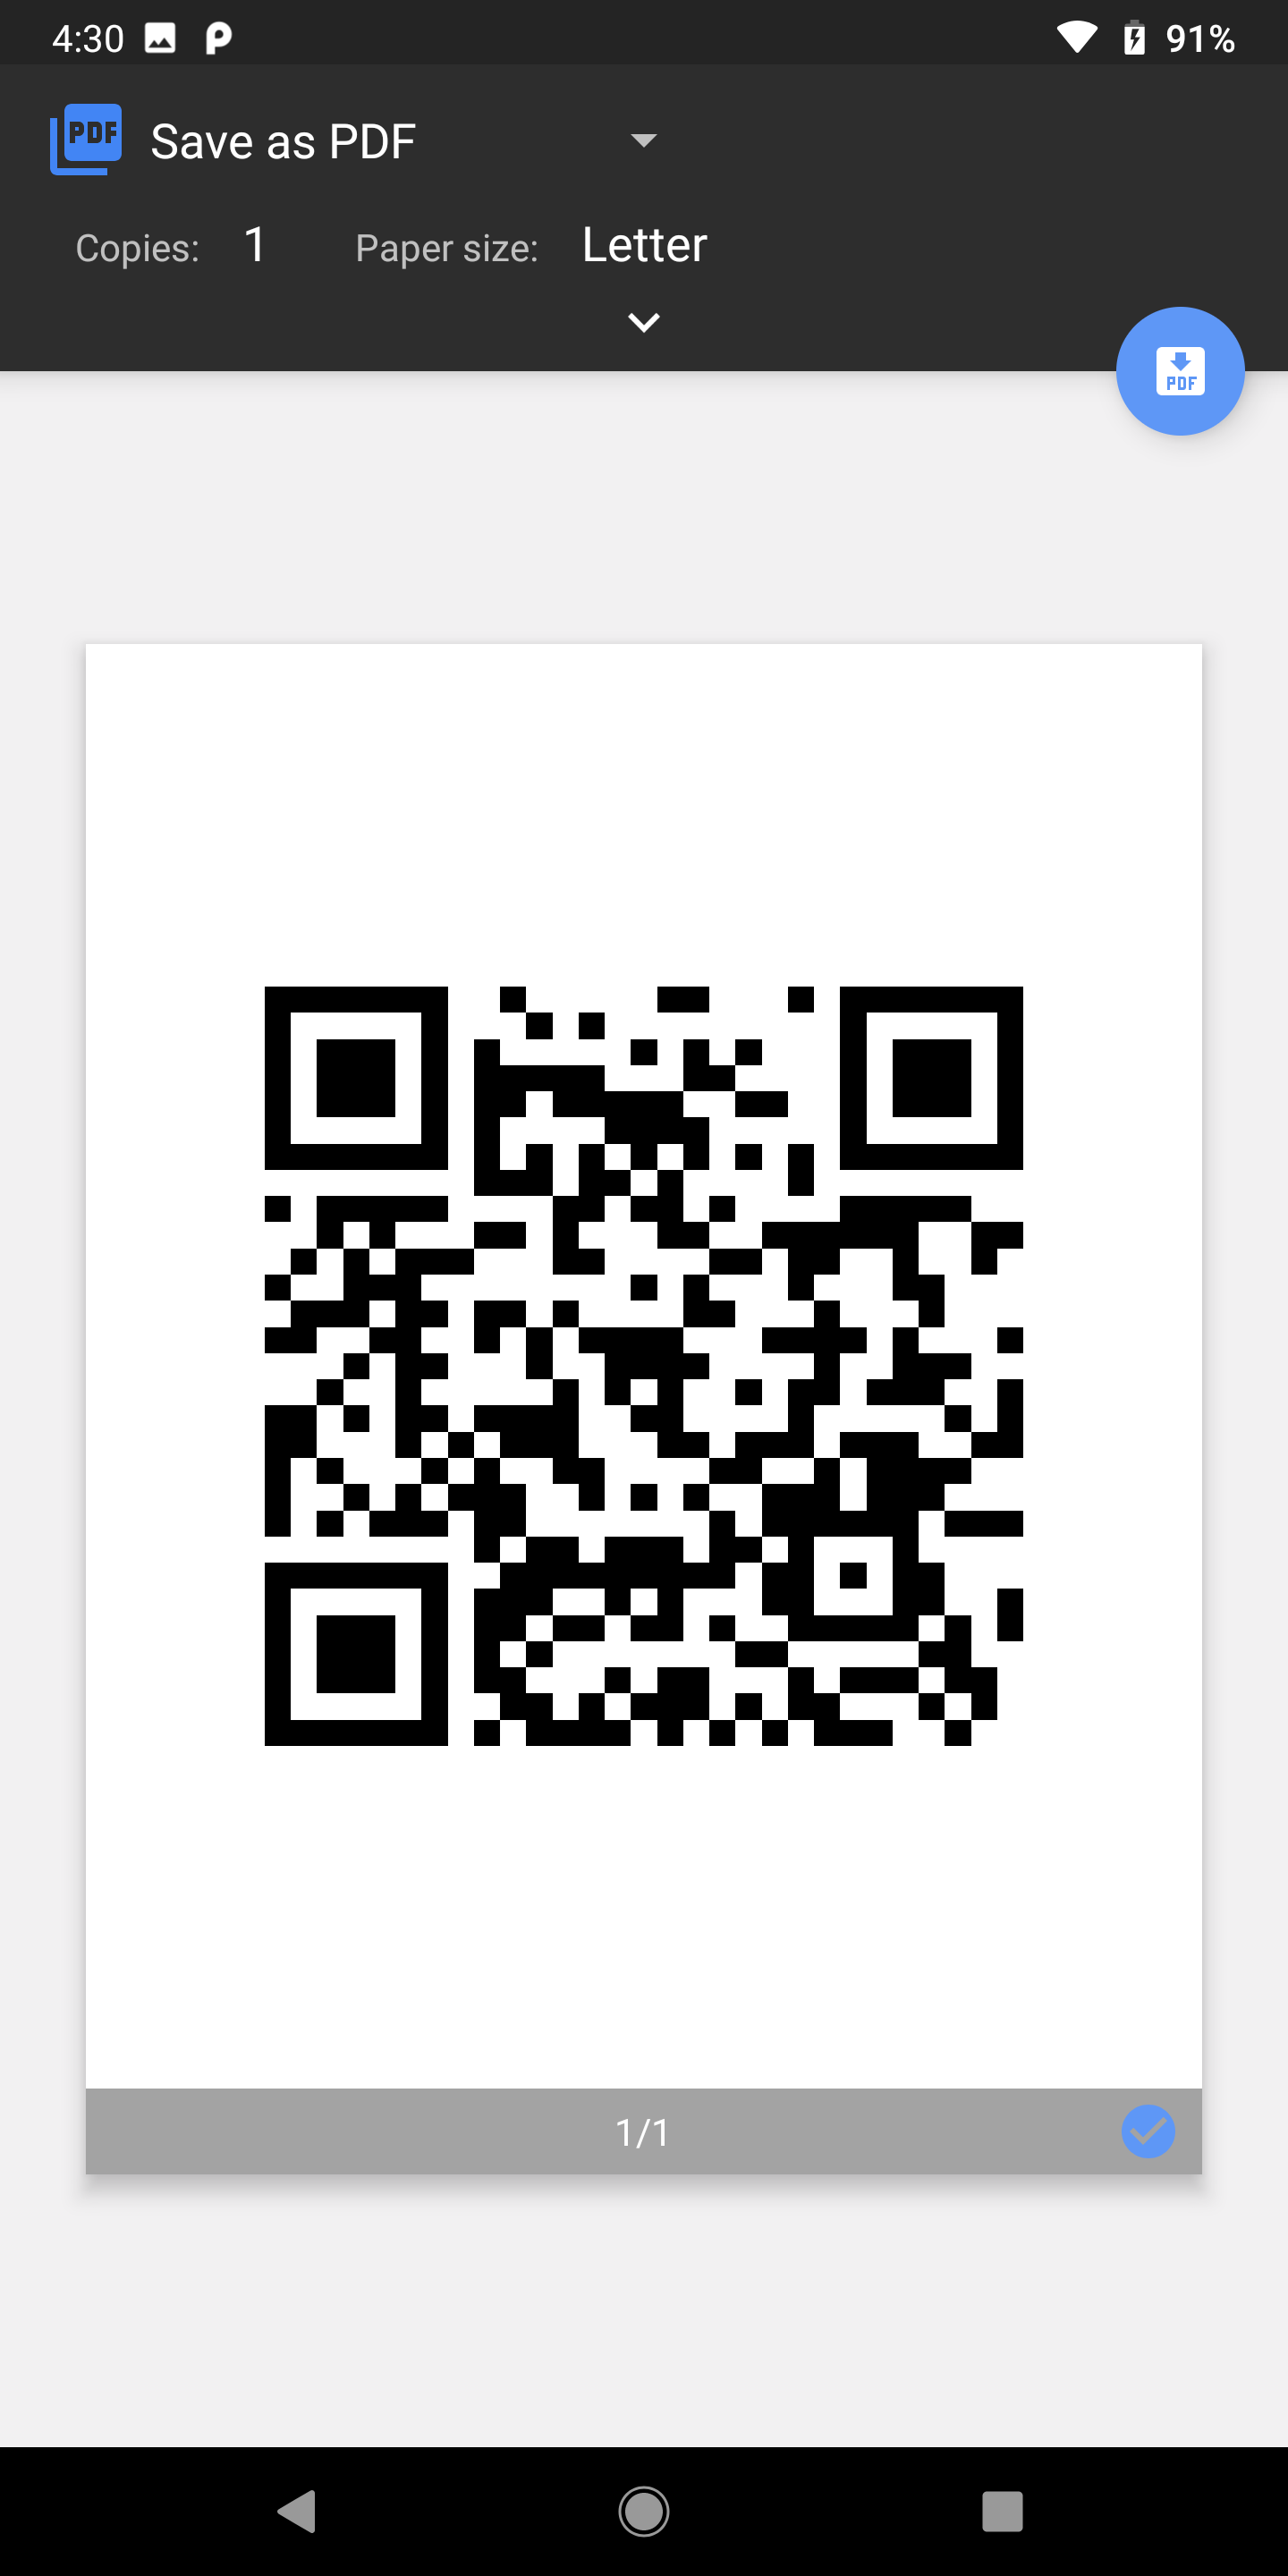
\includegraphics[height=8cm]{printing.png}
\end{frame}

\section{Features}
\begin{frame}
	\begin{center}
		{\Huge Which features will it have?}
	\end{center}
\end{frame}
\begin{frame}
  \frametitle{Features and division of labor}
  \begin{enumerate}
    \item Reading and creating QR codes, placing content and printing - Leon
    \item Displaying and playing web content dynamically and transparently - Jonathan
    \item Tracking and placing QR codes and displaying content relationally - Adrian
  \end{enumerate}
\end{frame}

\begin{frame}
  \frametitle{Work to be done}
  Functionality almost completely implemented.

  \begin{itemize}
    \item Integrate into one experience
    \item Browser to render webpage
    \item Documentation
  \end{itemize}
\end{frame}

\frame{\titlepage}

\end{document}
